\documentclass{amsdtx}
\usepackage[margin=.75in]{geometry}
\usepackage{graphicx}
\usepackage{float}
\usepackage{eqnarray,amsmath}
\usepackage{amssymb}
\usepackage{hyperref}
\usepackage{url}
\usepackage{xcolor}
\usepackage{cancel}
\usepackage{multicol}
\usepackage[Glenn]{fncychap}
%\usepackage{hyperref}


\usepackage{enumitem}

\title{\sc Fin Root Bonding Procedure}
\author{\sc C. Casebolt, M. Nichitiu | MIT Rocket Team}
\date{\sc Project Aurora}
\begin{document}
\maketitle    
\section{Abstract}
We describe how to perform the root bonding of composite fins onto a 6.1'' OD G10 fuselage, using the provided alignment jig.
\section{Materials}
\begin{itemize}
	\item G10 Mission Package Tube (Fuselage)
	\item 4 CF-layup fins
	\item Alignment Jig
	\item Epoxy/Hardener mixture, in correct ratios
	\item Level
	\item 4 Clamps, ideally 8 (see step 18)
	\item Large vice (Rkt Team Lab)
\end{itemize}
\begin{figure}[H]
\centering
~\kern-0.5cm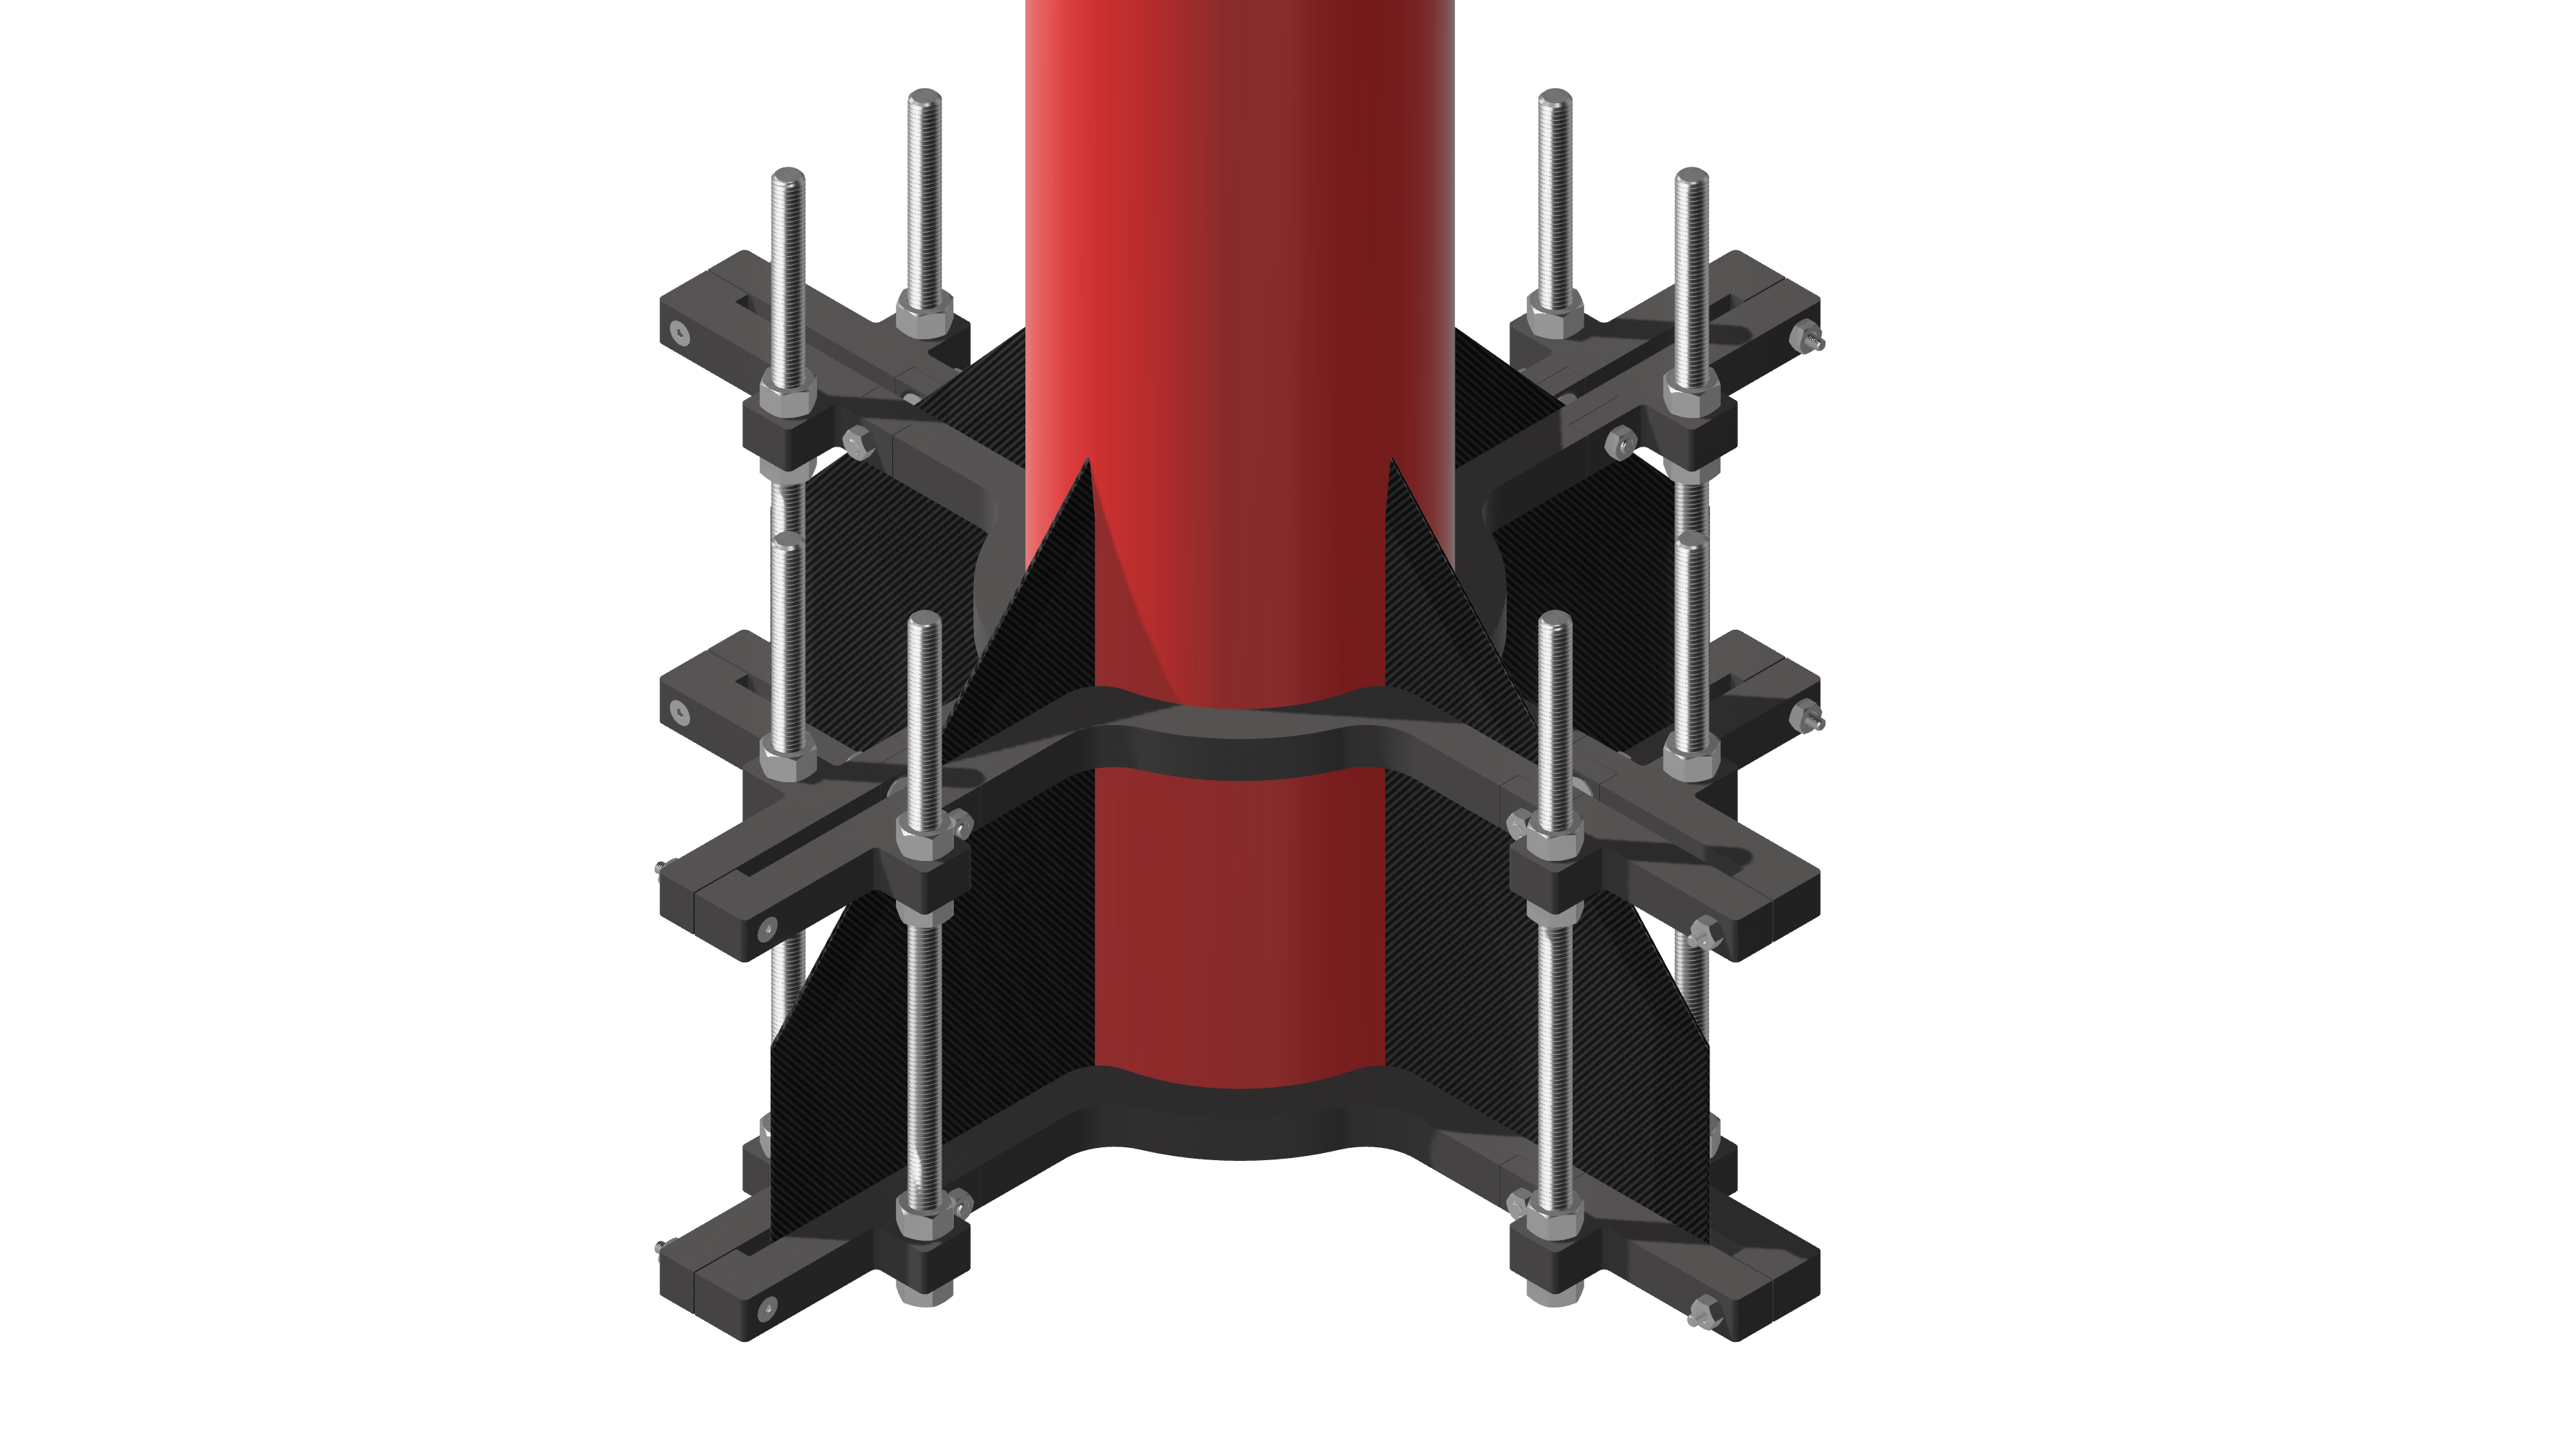
\includegraphics[scale=0.3]{render.png}
\caption{Fin Alignment Jig Setup.}	
\end{figure}
\section{Procedure}
\begin{enumerate}
	\item Begin by obtaining all materials.
	\item Label the branches of the jig as $A$, $B$, $C$, $D$, clockwise.
	\item Insert the G10 into the center of the jig, aligning the bottom of the G10 with the bottom of the 3D printed pieces (not the bottom of the bolts).
	\item Tighten the far screws on $A$ and $D$ to the maximum.
	\item Loosen the far screws on $B$ and $C$ slightly, so that a fin can be smoothly inserted. 
	\item Open the vice enough so that branch $A$ of the jig can fit in the vice, with the vice axis parallel to the G10 axis.
	\item Ensure that the bolts holding the axles have a flat side when resting on the vice holder. Tighten the interior bolts as needed to maintain grip on the 3D printed pieces.
	\item Tighten the vice until resistance is encountered, then one half turn more.
	\item Use a level to verify that the two axles closest to the vice (those of branch $A$) are parallel to the ground. Calibrate your level to this.
	\item Prepare the root chord of the fin that will enter in branch $B$ with the epoxy/hardener mix
	\item When ready, insert it into the branch $B$. 
	\item Then, tighten the screws on branch $B$ until resistance is encountered.
	\item Then, push the fin up to the G10, ensuring that the trailing edge is flush with the end of the 3D printed pieces, and the root chord is flush with the G10.
	\item Tighten the screws on branch $B$ fully, and use two of the clamps to eliminate space between the jig and the fin near the root chord (between the axle and the G10).
	\item Repeat steps 10 through 14 for branch $D$ and another fin.
	\item Let the epoxy harden.
	\item Confirm with the level that the fins in branches $B$ and $D$ are level according to the calibration.
	\item Repeat the steps 10 through 17, but this time with branch $B$ in the vice, using first branch $A$ and then $C$, and removing the clamps only if 4 clamps total could be found (but not loosening the screws).
	\item Once all fin bonding has hardened, remove the jig from the vice, remove all clamps, unscrew the external screws of each branch completely, and decompose the jig, leaving a root-bonded fin can. 
	\item Place this fin can in the vice (gently) and use a level to confirm that the angles are correct.
	\item Et voil\`a !
\end{enumerate}

\end{document}













